\chapter{Implementation}
\label{ch:implementation}

HRIStudio is a reference implementation of the design principles established in Chapter~\ref{ch:design}. The central contribution of this work is not the tool itself but the design concepts that underpin it: the hierarchical specification model, the event-driven execution model, and the integrated data flow. Any system built on those concepts would satisfy the same requirements. This chapter explains how HRIStudio realizes them, covering the architectural choices and mechanisms behind how the platform stores experiments, executes trials, integrates robot hardware, and controls access. Technology stack specifics are presented in Appendix~\ref{app:tech_docs}.

\section{Platform Architecture}

HRIStudio follows the model of a web application. Researchers access it through a standard browser without installing specialized software, and the entire study team, including researchers, wizards, and observers, connect to the same shared system. This eliminates the need for a local installation and ensures the platform works identically on any operating system, directly addressing the low-technical-barrier requirement (R2, from Chapter~\ref{ch:background}). It also enables easy collaboration (R6): multiple team members can access experiment data and observe live trials simultaneously from different machines without any additional configuration.

I organized the system into three layers: a browser-based user interface, an application server that manages execution, authentication, and logging, and a data and robot control layer covering storage and hardware communication. This layered structure is shown in Figure~\ref{fig:three-tier}. A key deployment constraint is that the application server runs on the same local network as the robot hardware. This keeps communication latency low during live trials: a noticeable delay between the wizard's input and the robot's response would break the interaction.

I implemented all three layers in the same language — TypeScript~\cite{TypeScript2014}, a statically-typed superset of JavaScript. The single-language decision keeps the type system consistent across the full stack. When the structure of experiment data changes, the type checker surfaces inconsistencies across the entire codebase at compile time rather than allowing them to appear as runtime failures during a live trial.

\section{Experiment Storage and Trial Logging}

The system saves experiments to persistent storage when a researcher completes them in the Design interface. A saved experiment is a complete, reusable specification that a researcher can run across any number of trials without modification.

When a trial begins, the system creates a new trial record linked to that experiment. The system writes every action the wizard triggers to that record with a precise timestamp, whether scripted or not, including any unscripted actions triggered outside the protocol. The system flags those unscripted actions as deviations. The browser records video, audio, and robot sensor data alongside the action log for the duration of the trial. The Analysis interface can directly compare what was planned against what was executed for any trial, without any manual work by the researcher, because the trial record and the experiment reference the same underlying specification. Figure~\ref{fig:trial-record} shows the structure of a completed trial record: action log entries, video, audio, and robot sensor data all share a common timestamp reference so the Analysis interface can align them without manual synchronization; dashed lines mark step boundaries; and the system flags any deviation from the experiment specification inline.

\begin{figure}[htbp]
\centering
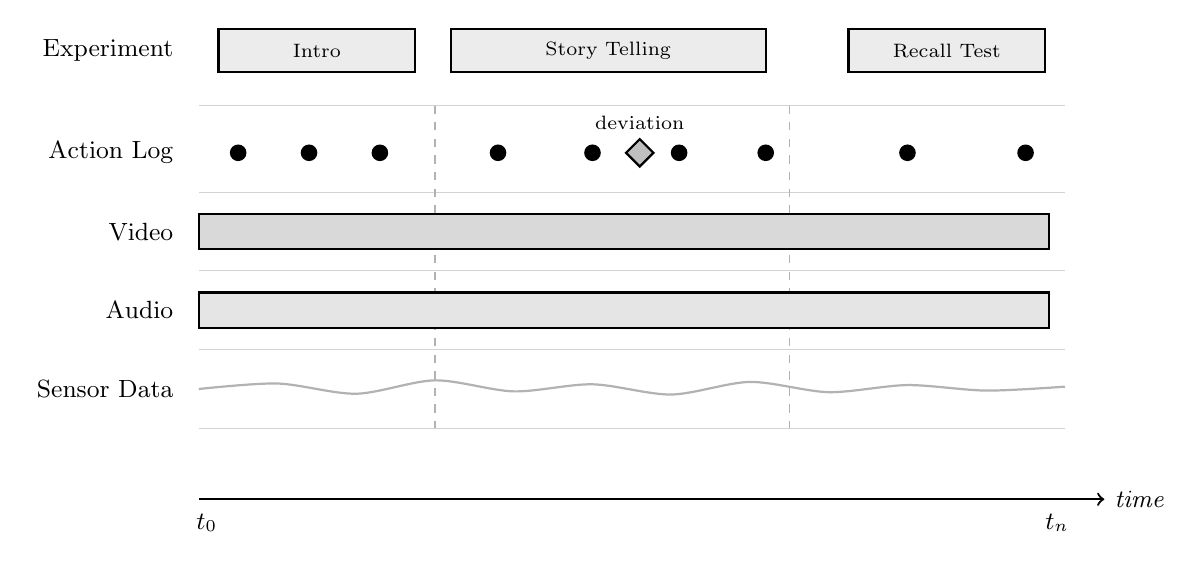
\begin{tikzpicture}[
    dot/.style={circle, fill=black, minimum size=6pt, inner sep=0pt},
    devdot/.style={rectangle, draw=black, thick, fill=gray!50, minimum size=7pt, inner sep=0pt, rotate=45},
    stepbox/.style={rectangle, draw=black, thick, fill=gray!15, align=center, font=\scriptsize, inner sep=3pt, minimum height=0.55cm},
    mediabar/.style={rectangle, draw=black, thick, fill=gray!30, minimum height=0.45cm},
    track/.style={font=\small, anchor=east}]

    % Time axis
    \draw[->, thick] (0, -0.5) -- (11.5, -0.5) node[right, font=\small\itshape] {time};
    \node[font=\small] at (0.1, -0.8) {$t_0$};
    \node[font=\small] at (10.9, -0.8) {$t_n$};

    % Track labels
    \node[track] at (-0.2, 5.2) {Experiment};
    \node[track] at (-0.2, 3.9) {Action Log};
    \node[track] at (-0.2, 2.9) {Video};
    \node[track] at (-0.2, 1.9) {Audio};
    \node[track] at (-0.2, 0.9) {Sensor Data};

    % Track dividers
    \foreach \y in {4.5, 3.4, 2.4, 1.4, 0.4} {
        \draw[gray!35, thin] (0, \y) -- (11.0, \y);
    }

    % Experiment step boxes
    \node[stepbox, minimum width=2.5cm] at (1.5, 5.2) {Intro};
    \node[stepbox, minimum width=4.0cm] at (5.2, 5.2) {Story Telling};
    \node[stepbox, minimum width=2.5cm] at (9.5, 5.2) {Recall Test};

    % Step boundary markers
    \draw[dashed, gray!60] (3.0, 4.5) -- (3.0, 0.4);
    \draw[dashed, gray!60] (7.5, 4.5) -- (7.5, 0.4);

    % Scripted actions
    \node[dot] at (0.5, 3.9) {};
    \node[dot] at (1.4, 3.9) {};
    \node[dot] at (2.3, 3.9) {};
    \node[dot] at (3.8, 3.9) {};
    \node[dot] at (5.0, 3.9) {};
    \node[dot] at (6.1, 3.9) {};
    \node[dot] at (7.2, 3.9) {};
    \node[dot] at (9.0, 3.9) {};
    \node[dot] at (10.5, 3.9) {};

    % Deviation marker
    \node[devdot] at (5.6, 3.9) {};
    \node[font=\scriptsize, above=5pt] at (5.6, 3.9) {deviation};

    % Video bar
    \node[mediabar, minimum width=10.8cm] at (5.4, 2.9) {};

    % Audio bar
    \node[mediabar, minimum width=10.8cm, fill=gray!20] at (5.4, 1.9) {};

    % Sensor data (continuous sampled line)
    \draw[thick, gray!60] plot[smooth] coordinates {
        (0.0, 0.90) (1.0, 0.97) (2.0, 0.84) (3.0, 1.01) (4.0, 0.87)
        (5.0, 0.96) (6.0, 0.83) (7.0, 0.99) (8.0, 0.86) (9.0, 0.95)
        (10.0, 0.88) (11.0, 0.93)
    };

\end{tikzpicture}
\caption{Structure of a completed trial record, showing synchronized action log, media, and sensor tracks.}
\label{fig:trial-record}
\end{figure}

Video and audio are recorded locally in the researcher's browser during the trial rather than streamed to the server in real time. This prevents network delays or server load from dropping frames or degrading audio quality during the interaction. When the trial concludes, the browser transfers the complete recordings to the server and associates them with the trial record. The Analysis interface can align video and audio with the logged actions without any manual synchronization, because the timestamp when recording starts is logged alongside the action log.

The system stores structured and media data separately. Experiment specifications and trial records live in a structured database, which makes it efficient to query across trials (for example, retrieving all trials for a specific participant or comparing action timing across conditions). Video and audio files live in a dedicated file store, since their size makes them unsuitable for a database and the system never queries their content directly.

\section{The Execution Engine}

The execution engine is the component that runs a live trial: it loads the experiment, manages the wizard's connection, dispatches robot commands, and keeps all connected clients in sync.

When a trial begins, the server loads the experiment and maintains a live connection to the wizard's browser and any observer connections. The execution engine does not advance the experiment on a timer; it waits for the wizard to trigger each step. This preserves the natural pacing of the interaction: the wizard advances only when the participant is ready, while the experiment structure ensures the protocol is followed. When the wizard triggers an action, the server dispatches the robot command, writes the log entry, and pushes the updated experiment state to all connected clients in the same operation — keeping the wizard's view, the observer view, and the actual robot state synchronized in real time.

No two participants respond identically. One subject gives a one-word answer; another offers a paragraph; a third asks the robot a question the script never anticipated. A fully programmed robot has no answer for that third subject: the interaction stalls, or immersion breaks. The wizard exists to fill that gap: where the program runs out of instructions, the wizard draws on their knowledge of human social interaction to keep the exchange coherent. Unscripted actions give the wizard the tools to exercise that judgment in the moment. The wizard triggers them via the manual controls in the Execution interface, the robot command runs, and the system logs the action with a deviation flag. This design preserves research value: the interaction gains the flexibility only a human can provide, and that flexibility appears explicitly in the record rather than disappearing into it.

\section{Robot Integration}

A configuration file describes each robot platform, listing the actions it supports and specifying how each one maps to a command the robot understands. The execution engine reads this file at startup and uses it whenever it needs to dispatch a command: it looks up the action type, assembles the appropriate message, and sends it to the robot over a bridge process running on the local network. The web server itself has no knowledge of any specific robot; all hardware-specific logic lives in the configuration file.

The execution engine treats control flow elements such as branches and conditionals the same way as robot actions. They appear as action groups in the experiment and resolve at runtime, so researchers can freely mix logical decisions and physical robot behaviors when designing an experiment without any special handling.

Figure~\ref{fig:plugin-architecture} illustrates this mapping using NAO6 and TurtleBot as an example. Actions a platform does not support (such as \texttt{raise\_arm} on TurtleBot) appear as explicitly unsupported in the configuration file rather than silently failing. The experiment itself does not change between platforms.

\begin{figure}[htbp]
\centering
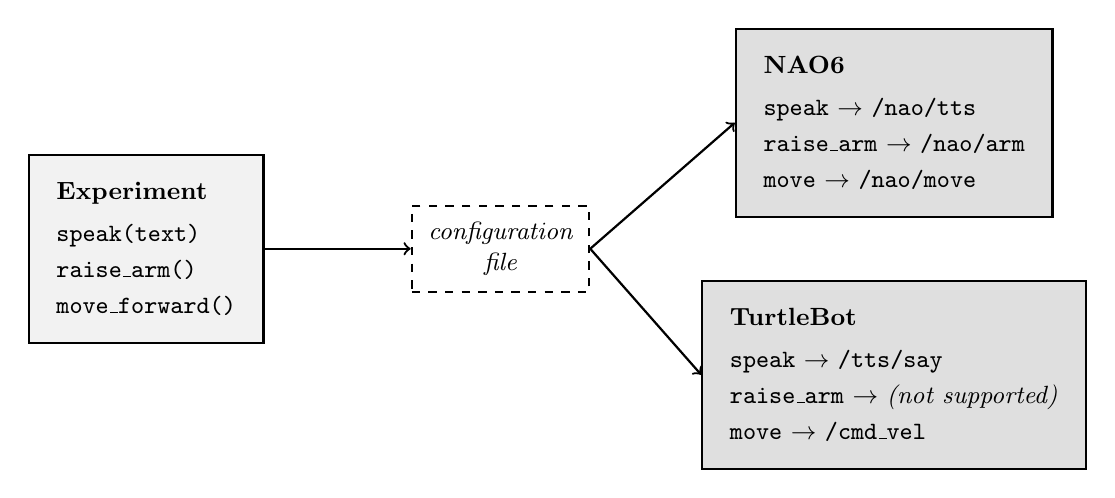
\begin{tikzpicture}[
    expbox/.style={rectangle, draw=black, thick, fill=gray!10, align=left, font=\small, inner sep=10pt},
    cfgbox/.style={rectangle, draw=black, thick, dashed, fill=white, align=center, font=\small\itshape, inner sep=6pt},
    robotbox/.style={rectangle, draw=black, thick, fill=gray!25, align=left, font=\small, inner sep=10pt},
    arrow/.style={->, thick}]

    % Experiment box
    \node[expbox] (exp) at (0, 0) {
        \textbf{Experiment}\\[4pt]
        \texttt{speak(text)}\\[2pt]
        \texttt{raise\_arm()}\\[2pt]
        \texttt{move\_forward()}
    };

    % Configuration file node (intermediate)
    \node[cfgbox] (cfg) at (4.5, 0) {configuration\\file};

    % NAO6 box
    \node[robotbox] (nao) at (9.5, 1.6) {
        \textbf{NAO6}\\[4pt]
        \texttt{speak} $\to$ \texttt{/nao/tts}\\[2pt]
        \texttt{raise\_arm} $\to$ \texttt{/nao/arm}\\[2pt]
        \texttt{move} $\to$ \texttt{/nao/move}
    };

    % TurtleBot box
    \node[robotbox] (tb) at (9.5, -1.6) {
        \textbf{TurtleBot}\\[4pt]
        \texttt{speak} $\to$ \texttt{/tts/say}\\[2pt]
        \texttt{raise\_arm} $\to$ \textit{(not supported)}\\[2pt]
        \texttt{move} $\to$ \texttt{/cmd\_vel}
    };

    % Arrows
    \draw[arrow] (exp.east) -- (cfg.west);
    \draw[arrow] (cfg.east) -- (nao.west);
    \draw[arrow] (cfg.east) -- (tb.west);

\end{tikzpicture}
\caption{Abstract experiment actions translated to platform-specific robot commands through per-platform configuration files.}
\label{fig:plugin-architecture}
\end{figure}

\section{Access Control}

I implemented access control using a role-based access control (RBAC) model. Each study has a membership list, and every member is assigned one of four roles that define a clear separation of duties: those who own the study, those who design it, those who run it, and those who observe it. This enforces need-to-know access at the study level so that each team member sees only what their role requires.

\begin{description}
    \item[Owner.] Full control over the study: can invite or remove members, configure the study settings, and access all data.
    \item[Researcher.] Can create and modify experiment designs and review all collected trial data, but cannot manage team membership.
    \item[Wizard.] Can trigger actions during a live trial and view the execution interface, but cannot modify the experiment design or access other wizards' sessions.
    \item[Observer.] Read-only access: can watch a live trial in real time and annotate significant moments, but cannot trigger actions or modify any data.
\end{description}

The role system also supports double-blind designs~\cite{Bartneck2024}: the Owner can restrict a Wizard's view of condition assignments, and restrict Researchers from accessing result data until the study concludes, without any changes to the underlying experiment.

\section{Architectural Challenges}

Two problems required specific solutions during implementation.

\begin{description}
    \item[Execution latency.] During a live trial, the execution engine must respond quickly to wizard input — a noticeable delay between the button press and the robot's action can disrupt the interaction. I addressed this by maintaining a persistent connection for the duration of each trial. The connection is established once at trial start and kept open, eliminating per-action setup overhead.

    \item[Multi-source synchronization.] Analysis requires aligning data streams captured at different sampling rates by different components: video, audio, action logs, and sensor data. The solution is a shared time reference: every data source records its timestamps relative to the same trial start time, $t_0$, so the Analysis interface can align all tracks without requiring manual calibration. This is the timestamp structure shown in Figure~\ref{fig:trial-record}.
\end{description}

\section{Implementation Status}

HRIStudio has reached minimum viable product status. The Design, Execution, and Analysis interfaces are operational. The execution engine handles scripted and unscripted actions with full timestamped logging, and I validated robot communication on the NAO6 platform during development. The platform can run a controlled WoZ study without modification.

Work remaining for future development includes support for studies that use more than one robot at a time and validation of the configuration file approach on robot platforms beyond NAO6.

\section{Chapter Summary}

This chapter described how HRIStudio realizes the design concepts from Chapter~\ref{ch:design} in practice. Experiments are persistent, reusable specifications that produce complete, comparable trial records. The execution engine is event-driven rather than timer-driven, keeping the wizard in control of pacing while logging every action automatically. Per-platform configuration files keep the execution engine hardware-agnostic. The role system enforces access control at the study level. The platform is at minimum viable product status and can run a controlled WoZ study today. HRIStudio is one realization of these concepts; the contribution lies in the design principles themselves, which any implementation could adopt.
